%---------------------------------------------------
%---------------------------------------------------
%-----   COPY FROM HERE TO DEFINITIVE FILE    ------
%---------------------------------------------------
%---------------------------------------------------


\clearpage{\pagestyle{empty}\cleardoublepage}


\chapter{LHC and the ATLAS experiment}\label{chap:atlas}
%Since before the Large Electron Positron Collider (LEP) started runs in 1989, scientists were thinking about making the most of the 27-kilometer long tunnel by building a more powerful collider.

In 1994, the CERN Council approved the Large Hadron Collider (LHC) project and two years later official approval came also for the experiments ATLAS and CMS, followed in 1997 by ALICE and in 1998 by LHCb. The aim in building a proton-proton collider able to reach a center of mass energy above 10 TeV is to go further in the new physics sector after Tevatron's results, including the long awaited discovery of the Higgs boson.

The Large Electron Positron Collider (LEP) ended its activity in year 2000 and was dismantled to give up its place in the 27-kilometer long tunnel to LHC, which by 2008 was fully installed and ready to start. On 10th September 2008 the first beams were circulated successfully in the LHC. After nine days of running, on the verge of getting the first collision at $\sqrt{s} = 900$~GeV, a serious accident happened causing bad damages to the accelerator. This stopped the activities and the first half of 2009 was devoted to repair the damage and improve the safety of operations.

The LHC started to run again on the 20th of November 2009 after more than one year after the accident. During this long time the damage has been repaired and security has been improved as well. The performance of the machine in the first weeks of running are very promising, and we report a little piece taken from the CERN news\footnote{\url{http://press.web.cern.ch/press/PressReleases/Releases2009/PR18.09E.html}} of ten days after the restart:
\begin{quotation}\small
Geneva, 30 November 2009. CERN's Large Hadron Collider has today become the world’s highest energy particle accelerator, having accelerated its twin beams of protons to an energy of 1.18 TeV in the early hours of the morning. This exceeds the previous world record of 0.98 TeV, which had been held by the US Fermi National Accelerator Laboratory’s Tevatron collider since 2001. It marks another important milestone on the road to first physics at the LHC in 2010.
\end{quotation}


\section{The collider}
The LHC is a proton-proton collider that will be able to reach a center of mass (c.m.) energy $\sqrt{s}$ of 14 TeV, about 7 times Tevatron's c.m. energy. The main difference between the two colliders is that Tevatron was a proton-antiproton collider. This allowed to use only one ring since protons and antiprotons are of opposite charge and so the same field accelerates them in two opposite directions. In spite of this great advantage, antiprotons are difficult to produce and stock in big quantities, thus putting a limit on the achievable luminosity. Thus the choice to circulate two proton beams in two different rings was adopted. The proton bunches are then made to collide at the intersections of the rings where the experiments are placed (Figure \ref{lhc}).
\begin{figure}[htb]\begin{center}
\includegraphics[width=.47\textwidth]{capATLAS/hadron}\hspace{.01\textwidth}\includegraphics[width=.5\textwidth]{capATLAS/map}\caption{Computer generated image of the LHC tunnel with aerial view of the CERN site (left) and a picture of the underground placement of the experiments (right).}\label{lhc}
\end{center}\end{figure}
%\begin{figure}[htb]\begin{center}\includegraphics[width=.48\textwidth]{capATLAS/dipole}\includegraphics[width=.48\textwidth]{capATLAS/dipmag_diagram}\caption{Views of LHC dipole. }\label{dipole}\end{center}\end{figure}

The main performance figure for a Collider is the luminosity $\mathcal L$, defined as 
\begin{equation}\label{eq:lumiN}
\dfrac{dN}{dt} = \mathcal L \sigma ,
\end{equation} 
where $dN/dt $ is the event rate and  $ \sigma$ is the cross section of the process one wants to produce.
Integrating over the time in which the accelerator is active yields
the \textit{integrated luminosity}, relating the total number of produced
events $N$ to the cross-section:
\begin{equation}\label{eq:intLumi}
\int \mathcal L dt  = \dfrac{N}{\sigma} 
\end{equation}
It is clear that a high $\mathcal L$ and a long enough time interval of data taking would give us a great number of events, in spite of low cross sections. Figure \ref{xsec} shows the cross sections for different processes of interest as functions of the c.m. energy. Since the c.m. energy reachable is limited\footnote{There is a linear dependence between the magnetic field strength required to circulate the particle beams and the beam energy. The formula $$p\mbox{[TeV]} = 0.3B\mbox{[Tesla]}R\mbox{[km]}$$ for a beam momentum $p$ of 7 TeV and a ring radius $R \simeq 4.3$ km would give a value for the magnetic field $B$ about 5.4 Tesla, that in practice has to be increased to 8.4 in order to obtain the same bending power with a limited number of magnets.} by the affordable magnetic field (8.65 Tesla for the superconducting magnets), in order to increase the rate of events with interesting physics one has to increase luminosity through the choice of collider's parameters.

\begin{figure}[htb]\begin{center}
\includegraphics[width=.8\textwidth]{capATLAS/xsect.png}\caption{Expected cross sections for proton-proton collisions as functions of $\sqrt{s}$. (From \cite{hep})}\label{xsec}\end{center}\end{figure} 

To see the kind of luminosity required for reaching the LHC goals, let's
consider for example the production of a Higgs boson.
In this case,  the number of observable events is given by
\begin{equation}\label{eq:NEvent}
N_{\mbox{obs}} = \mathcal L\ \sigma\ BR\ \epsilon\ \Delta t,
\end{equation}
where $BR$ is the branching ratio of the selected decay, $\epsilon$ is the detector efficiency and $\Delta t$ is the time of running (a standard year at the LHC is supposed to be an effective running time of $10^{7}$ s). For an Higgs particle with mass around $100 -150$~GeV and decaying $H \rightarrow \gamma\gamma$ we have \cite{slideGiacomo}
\begin{equation}\label{eq:higgs1}
\sigma BR \epsilon \sim 10-20 \mbox{ fb}
\end{equation}
and the ratio S/B is about 1/50. Since S/$\sqrt{\mbox{B}} >$ 5 is required for discovery, a number of more than 1000 $H \rightarrow \gamma\gamma$ events is needed, meaning an integrated luminosity of $100$ fb$^{-1}$ i.e. one year of data taking at high luminosity $\mathcal L = 10^{34}$ cm$^{-2}$ s$^{-1}$.
%!!ESEMPIO DA SLIDE GIACOMO!!
%\begin{figure}[htb]\begin{center}\includegraphics[width=.45\textwidth]{capATLAS/bunches}\caption{A bunch crossing frequency of 40 MHz is needed for the high luminosity phase. (From \cite{slideGiacomo})}\label{bunch}\end{center}\end{figure}

The luminosity $\mathcal L$ for an intersecting storage ring collider 
is related to the machine parameters by the equation:
\begin{equation}\label{eq:lumi}
\mathcal L = f \dfrac{n_{1}n_{2}}{4\pi A_{x}A_{y}},
\end{equation}
where $n_{1}$ and $n_{2}$ are the number of particles in the two beams, $A_{x}$ and $A_{y}$ are the beam $x$ and $y$ dimensions assuming a Gaussian distribution for particles and $f$ is the collision frequency. 

Given the maximum achievable number of particles per bunch 
and the minimum beam size, 
in order to achieve the high required luminosity, the LHC  has
to run at a frequency of 40~MHz, which means that there is a beam crossing
in a detector every 25~ns.\par
The beam configuration (Table~\ref{tab:LHCpar}) is responsible for the pile-up phenomenon (see Section \ref{sec:LHCprobl}) and detectors have to satisfy specific requirements to cope with it. Considering LHC operative parameters at design luminosity (Table \ref{tab:LHCpar}) and a inelastic\footnote{Elastic scattering of protons and diffractive events will not be detected since only particles from inelastic processes are emitted at angles with respect to the beam axis high enough to be seen from detectors.} proton-proton cross section $\sigma_{\mbox{tot}} \sim 70$ mb, an event rate  $\mathcal L\sigma_{\mbox{tot}}$ of about $10^{9}$ interactions per second is expected. This means that for every bunch crossing about 25 events are superimposed and around 1000 charged tracks will be produced from the collision within the pseudorapidity region $|\eta| < 2.5$.
%NB capire meglio da dove salta fuori quel 1000!!!!!!!!!

\begin{table}[htb]\centering\begin{tabular}{ccc}
\multicolumn{3}{c}{LHC operative parameters}\\ \midrule
$\mathcal L$ (low phase) & protons/bunch & collision rate\\ 
10$^{33}$ cm$^{-2}$s$^{-1}$ & $10^{11}$& 40 MHz \\\midrule
$\mathcal L$ (high phase) & bunch number & bunch crossing \\ 
10$^{34}$ cm$^{-2}$s$^{-1}$ & 2835 & 25 ns \\\hline\hline\end{tabular}\caption{Summary of LCH operative parameters.}\label{tab:LHCpar}\end{table}


%It is to notice that while at LEP the center of mass energy $\sqrt{s}$ was the effective center of mass energy for the interaction $e^{+}e^{-}$, at the hadron collider protons interact through the quarks they are composed of, and quarks carry only a fraction of the proton energy given by the parton distribution function (pdf) which is not known theoretically but can only be studied in deep inelasting scattering experiments. Assuming that $x_{1}$ and $x_{2}$ are the fraction of momentum carried by the quarks (or gluons) 1 and 2, the effective c.m. energy for the interaction is\begin{equation}\label{eq:cmenergy}
%\sqrt{s'} = \sqrt{x_{1}x_{2}s}.
%\end{equation} The proton is composed by up and down quarks that are the \textit{valence quarks} but it contains also gluons and other \textit{sea quarks} that, even if carrying a lower fraction of momentum, can interact at short distance (i.e. high exchanged momentum $q^{2}$). Sea quark are mainly produced by gluon radiation and gluon splitting into $q\bar{q}$ pairs.


\subsection{Physics Motivations}\label{sec:physMot}

%The LHC project comes from strong physics motivations\footnote{See also Chapter \ref{chap:Susy}.} that can justify the big economical and human effort besides the high technological complexity. 
The main aim of the LHC project, justifying the huge economical and human investment by more than 4000 pysicists working in the LHC collaboration is the discovery of the Higgs boson. This discovery would verify  the model  of Spontaneous Symmetry Breaking (SSB) or Higgs mechanism accounting for the origin of particle masses within the Standard Model. The mass of the Higgs boson is not predicted from theory but it is contrained under 1 TeV (in order to preserve unitarity at high energy) and above 120~GeV (from experimental limits from direct searches experiments from previous accelerators, see e.g. Ref. \cite{Renton}). The LHC experiments are designed in such a way that if the Higgs exists, the LHC will be able to observe it over this full mass range.

Besides the exploration of the Electroweak symmetry breaking mechanism, the LHC will hunt for physics going beyond the present accepted paradigm, the Standard Model, which might manifest itself in the new energy range opened to exploration by the LHC.

Furthermore, LHC will be able to perform precision measurements suitable for getting more details about known particles and interactions with the highest achievable accuracy. This is important for collection of more informations about the possible backgrounds for unknown processes as well as for finding eventually deviations from the Standard Model that are hints for new physics. For example, LHC is a ``top factory'', i.e. the top quark, the less well known quark, is going to be copiously produced at a rate of few tens of Hz and thus more precise measurements of its properties will be possible.

Finally, there are many open questions, somehow related to the previous topics, that could find an answer from LHC data. The origin of the universal asymmetry between matter and antimatter, the composition of dark matter, the origin of the QCD confinement and studies of a quark-gluon plasma state\footnote{A second stage of operation schedules the circulation of heavy ions beams at a c.m. energy of 11 TeV and luminosity of $10^{27}$ cm$^{-2}$s$^{-1}$.} are only some of the challenges which face the LHC expriments.


\subsection{Experimental Challenges}\label{sec:LHCprobl}

The events of interest such as ones producing high mass objects (i.e. high $p_{T}$ events) are often covered by the dominating QCD-jet processes. While detailed studies of QCD are an interesting goal \textit{per se}, they are believed to contain little unknown physics and are therefore regarded as background to new physics searches.

As can be seen from Figure \ref{xsec}, the total cross section and the cross section for interesting physics processes can differ for more than ten orders of magnitude. In fact, signal processes mostly involve heavy particles ($\sigma_{\tilde{q}\tilde{q}} \sim 1$ pb for masses $m(\tilde{q})$ more than 1 TeV) and/or have weak cross sections ($\sigma_{\mbox{\scriptsize Higgs}} \sim $ 30~pb for an Higgs mass of 100~GeV).
The bulk of the interaction cross-section is however given by
the so called \textit{minimum bias events}. Generally speaking, minimum bias events are soft interactions (low energy transfer in collision) with small transverse momentum ($p_{T} \sim 500$~MeV) and large longitudinal momentum with respect to the beam pipe direction, resulting in events with many hadrons of low momentum and nothing else in the detector.
Even requiring the presence of high momentum particle, one would be dominated by QCD,  as the QCD cross section is $\sigma_{\mbox{\scriptsize jets}} \sim \mu$b for jets with a transverse energy higher than 100~GeV. 

In order to separate interesting events from the overwhelming background clear signatures are required like the identification of leptons with high transverse momentum. In fact leptons have a very low rate in QCD events while are often present in interesting decay modes of the desired physics processes. Thus the design of the detectors is  driven by the online selection and identification of final states involving $\gamma$, leptons, missing transverse energy, $b$-jets which can be separated from QCD.

The other experimental difficulty is the pile-up: as mentioned before, at high luminosity every 25~ns about 25 soft interactions occur generating something like 1000 charged tracks. If one of the rare interesting processes is also emerging from the collision at a given crossing, it is going to be overlapped with the 25 minimum bias events. Figure \ref{higgsevent} shows a simulated Higgs boson decaying into four muons completely hidden it the crowd of tracks. However if a cut on the transverse momentum is applied requiring $p_{T}>25$~GeV, then the four lepton signature becomes clearly visible. \begin{figure}[htb]\begin{center}
\includegraphics[width=.6\textwidth]{capATLAS/higgsevent}\caption{$H\rightarrow 4\mu$ event in CMS at high luminosity. (From \cite{slideGiacomo})}\label{higgsevent}
\end{center}\end{figure}

Pile-up is a severe problem and implies three important choices about detector design. In fact a fast response is needed in order to avoid the integration over many bunch crossing with the result of adding up multiple pile-up. Typical response times are of 20-50 ns, thus integrating over 1-2 bunch crossings (and summing 25-50 minimum bias events). For this purpose a very high performing readout electronics is needed. Secondly, LHC detectors require a fine granularity thus minimising the probability for an interesting object to go through the same detector element as pile-up particles. This means a large number of electronic channels, increasing the cost and the difficulty of detector operations like calibration and monitoring. Finally there is a crucial requirement about radiation hardness of the detector, since the high flux of particles from the proton-proton collisions creates an high radiation environment. For instance, 10 years of operation mean an integrated flux of up to 10$^{17}$ neutrons per cm$^{2}$ and up to 10$^{7}$ Gy. This implies the possibility of severe damages to the detector composition, especially for the detectors near to the beam pipe: it is then fundamental to have radiation resistant detector technology and electronics.

\section{The LHC experiments}
LHC has eight  interaction points where the two proton beams can be made to cross, and in four of these point four different experiments are placed (see Figure \ref{map}): two general purpose experiments (ATLAS, A Toroidal LHC ApparatuS, and CMS, Compact Muon Solenoid) and two dedicated experiments (LHCb, Large Hadron Collider Beauty, and ALICE, A Large Ion Collider Experiment). The webpages of the four Collaborations are listed in Ref.~\cite{webEXP}.
\begin{figure}[htb]\begin{center}
\includegraphics[width=.65\textwidth]{capATLAS/ring}\caption{Interaction points around the LHC ring. Experiments are located between 50 m and 150 m underground.}\label{map}
\end{center}\end{figure}

A general purpose detector has typically a layered structure dictated by the physical laws of radiation penetration (Figure \ref{interact}).
\begin{figure}[htb]
\begin{center}
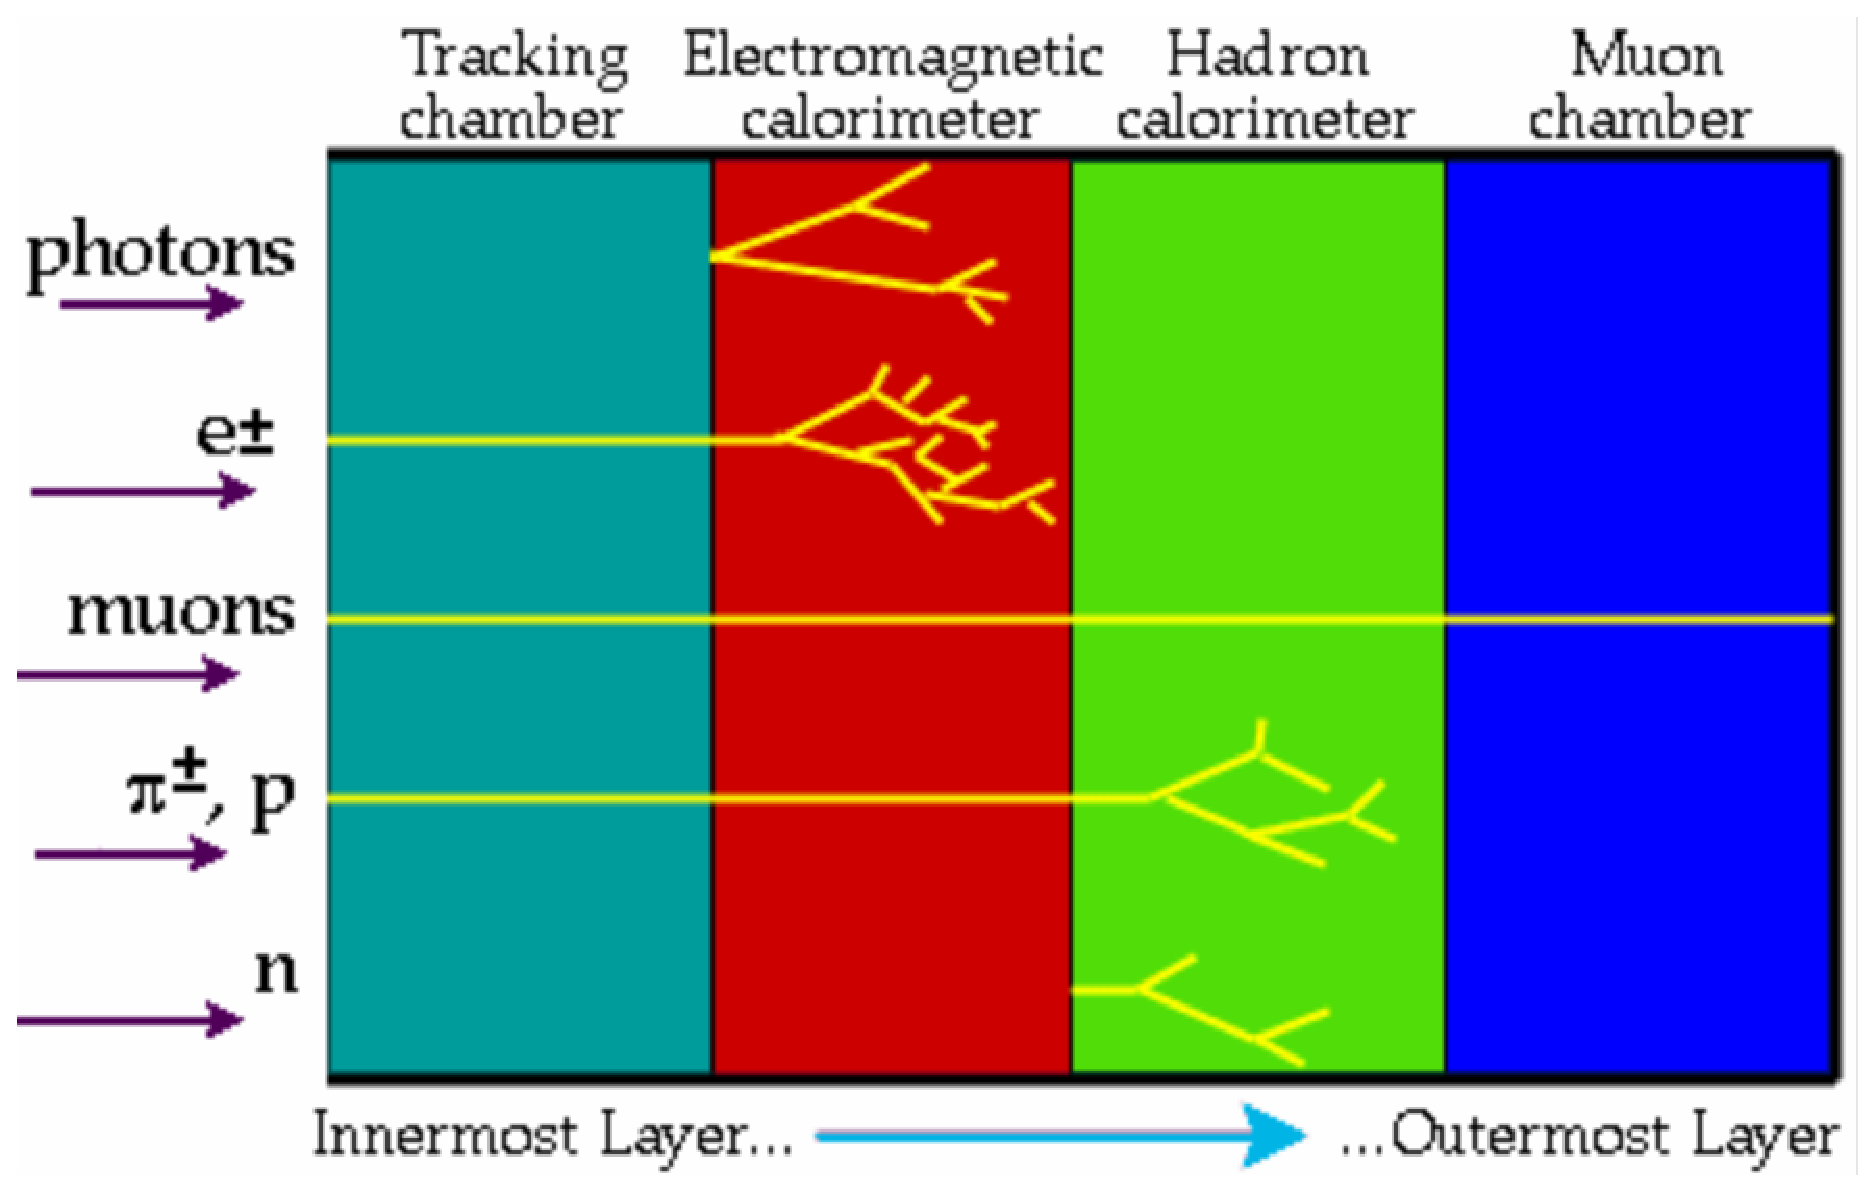
\includegraphics[width=.6\textwidth]{capATLAS/decay_chart}
\caption{Interaction of different particles in the different parts of the detector.}
\label{interact}
\end{center}
\end{figure} 
Such structure (from the interaction point to outside) consists of a vertex detector, a central tracker, an electromagnetic calorimeter, an hadronic calorimeter and a muon spectrometer. Based on this generic pattern the choice of technology and performance for the different components is dictated by the physics goals. In the case of general purpose detectors which are set to explore a new energy domain, it is mandatory to have detectors able to see as many particles and signatures as possible, since it is unknown how new physics is eventually going to manifest itself.

The standard coordinate system in a collider geometry has the $z$-coordinate along the beam. The direction of a particle is defined in term  of the azimuthal angle phi $\phi$ (in the $x-y$ plane), and the pseudorapidity $\eta$, defined as
\begin{equation}\label{eq:pseudoR}
\eta = -\log \bigg( \tan \dfrac{\theta}{2} \bigg),
\end{equation} 
where theta is the angle of the particle with respect to the $z$-axis.
A useful measure of the distance between two particles which will
be used in the analysis is given by: 
\begin{equation}
\label{eq:deltaR}
\Delta R = \sqrt{\Delta^{2}\eta + \Delta^{2}\phi}.
\end{equation} 
This definition of distance has the advantage to be invariant under a boost along the $z$-axis direction.


\subsection{Basic performance requirements}
LHC detectors have to be able to measure the transverse momentum of leptons in the range from a few~GeV up to few TeV in order to be sensitive to soft leptons from B-hadrons as well as to hard leptons from heavy ``new'' particles.

An high ermeticity is required for calorimetry such that the full azimuthal angle and the pseudorapidity region $|\eta| \leq 5$ are covered. This is motivated by the need to detect forward jets produced togeter with the Higgs boson in vector boson fusion processes, and to measure precisely the balance of momentum in the transverse plane. The latter point implies the possibility to reveal  particles like neutrinos which do not interact in the detector through a measurement of the missing transverse energy $\slashed{E}_{T}$\footnote{This comes from the simple kinematical argument of energy conservation stating that the initial total energy for the interacting quarks (or gluons) in the direction transverse to the beam line is ideally zero, while the same quantity along the Z axis is not predictable because of the unknown parton distribution functions.}. 
%This obviously implies that energy losses due to a poor coverage of the interaction region have to be minimised.

A mass resolution $\sim 10$\% for jet-jet invariant mass  of the order of one hundred~GeV, and of $\sim 1$\% for $\gamma\gamma$ and lepton-lepton invariant masses are needed in order to be able to detect resonance peaks above a continuum background. 

Furthermore a LHC detector must be able to reject jets faking electrons by a factor of $\sim 10^{5}$ in order to be able to detect an inclusive electron signal, considering that at the LHC the ratio $e$/jets ($p_{T} > 20$~GeV) between inclusive rates is $\sim 10^{-5}$. Similarly jets faking photons have to be rejected by a factor of $\sim 10^{3}$ for a photon efficiency of $\sim$80\%.

Finally the trigger system has to select an amount of data suitable to be stored. The target rate is  100 event recorded per second, out of the $10^{9}$ total events per second at high luminosity. Thus a rejection rate of $10^{7}$ is needed combined to a fast response, meaning a very selective and efficient trigger. 


\section{The ATLAS detector}
The design of the ATLAS experiment (shown in Figure \ref{atlas}) is optimised simultaneously for known, hypothetical and totally new processes. In fact the detector was built having specific processes in mind but it is also well prepared for the discovery of completely new phenomena. 
\begin{figure}[htb]\begin{center}
\includegraphics[width=.9\textwidth]{capATLAS/atlas}\caption{Overall design of the ATLAS detector. }\label{atlas}
\end{center}\end{figure}

The right-handed coordinate system with the $x$-axis pointing towards the centre of the LHC tunnel, the $y$-axis slightly different from vertical because of the general tilt of the LHC tunnel and the $z$-axis along the tunnel is shown in  Figure~\ref{coord}. In the pseudorapidity defininition (Eq. \ref{eq:pseudoR}) $\theta$ is the polar angle of the particle direction measured from the positive $z$-axis, while the transverse components are the perpendicular to the LHC beam axis. Different regions in the $z-y$ plane are defined through the pseudorapidity $\eta$ (some values are reported in Table \ref{tab:etatheta} with the corrispondent angle): the region with $|\eta|< 1$ is called \textit{barrel} or \textit{central region}, while regions with $|\eta|> 1$ are generally named \textit{forward regions} (see Figure \ref{regions}). Besides ATLAS has a symmetry forward-backward, the centre of symmetry being the interaction point and centre of coordinate system. The detector region on the positive side of the $z$-axis and forward region is called ``side A'', while the symmetric part on the negative $z$-axis is the backward region called ``side C'' (Figure \ref{coord}).

\begin{figure}[htb]\begin{center}
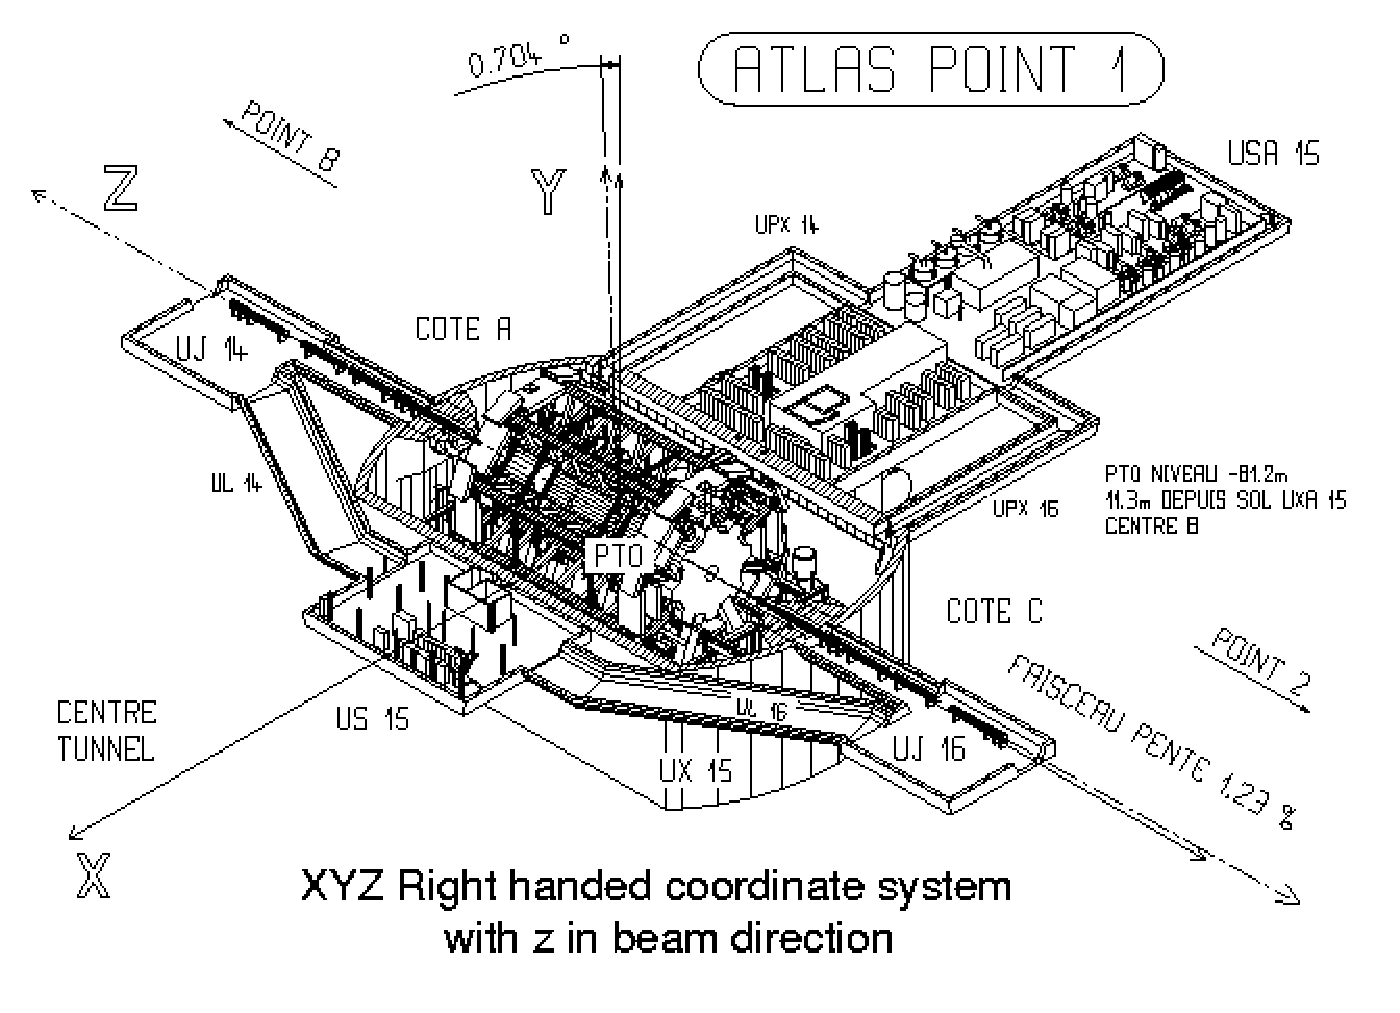
\includegraphics[width=.6\textwidth]{capATLAS/coord}\includegraphics[width=.3\textwidth]{capATLAS/Pseudorapidity}
\caption{Coordinate system with respect to the ATLAS detector (From \cite{hep}) and pseudorapidity. The $z$-axis is along beam direction while the $x$-axis points towards the centre of the ring.}
\label{coord}\end{center}\end{figure}

\begin{table}[htb]\centering\begin{tabular}{cccccccccc}\hline
$\theta$ & 0$^{\circ}$ & 5$^{\circ}$ & 10$^{\circ}$ & 20$^{\circ}$ & 30$^{\circ}$ & 45$^{\circ}$ & 60$^{\circ}$ & 80$^{\circ}$ & 90$^{\circ}$ \\
$\eta$ & $\infty$ & 3.13 & 2.44 & 1.74 & 1.31 & 0.88 & 0.55 & 0.175 & 0\\\hline\hline \end{tabular}\caption{Pseudorapidity values.}\label{tab:etatheta}\end{table}

\begin{figure}[htb]\begin{center}
\includegraphics[width=.3\textwidth]{capATLAS/regions1}\hspace{.5cm}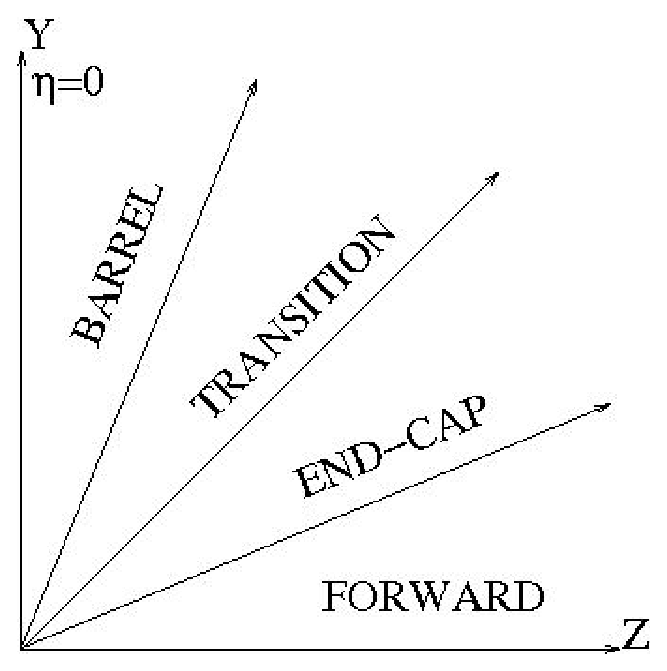
\includegraphics[width=.3\textwidth]{capATLAS/regions2}\caption{Pseudorapidity regions. The $z$-axis is along beam direction.}\label{regions}
\end{center}\end{figure}

The detector is a cylinder with a total length of 44 m and diameter of 25 m, with a double configuration of magnets. A superconducting solenoid producing a 2 Tesla field is close to the interaction point while three toroids (one barrel and two end-caps of 0.5-1 Tesla respectively) cover the outermost part of the detector.

The system of inner detector is 6.2 m long, has an outer radius of 1.05 m and is placed inside the superconducting solenoid. It is composed by silicon detectors (closest to the interaction point) and a straw tube tracker (outside them) that is also a transition radiation detector.

Outside the solenoid coil there is the liquid Argon (LAr) electromagnetic sampling calorimeter, made of layers of lead and liquid Argon. The hadronic calorimeter is a scintillator tile calorimeter in the barrel region up to $|\eta|<1.7$ while in the end-caps it is again a LAr sampling calorimeter. In the forward regions LAr sampling calorimeters act as electromagnetic and hadronic calorimeters covering a range of pseudorapidity up to $|\eta|<4.9$. %The total dimensions of the calorimeter is 2.25 m in radius and a half length of 6.65 m.

In the outermost part of the ATLAS detector, combined to the air core toroid magnetic system, there are the muon drift chambers, arranged in three layers. Table \ref{tab:performance} shows the main general performance goals for the ATLAS detector design.

\begin{table}[htb]\centering\begin{tabular}{ccccc}
\multicolumn{2}{c}{\multirow{2}*{Detector component}} & \multirow{2}*{Required resolution}& \multicolumn{2}{c}{$\eta$ coverage}\\
&&&Measurement &Trigger\\\midrule
\multicolumn{2}{c}{Tracking} & $\dfrac{\sigma_{p_{T}}}{p_{T}} = 0.05\% p_{T} \oplus1\%$ & $ \pm2.5$ & \\\midrule
\multicolumn{2}{c}{EM calorimetry} &$\dfrac{\sigma_{E}}{E} = \dfrac{10\%}{\sqrt{E}} \oplus0.7\%$ & $\pm3.2$ & $ \pm2.5$ \\\midrule
\multirow{2}*{H calo} &barrel,end-cap &  $\frac{\sigma_{E}}{E}= \frac{50\%}{\sqrt{E}} \oplus3\%$ & $\pm3.2$ & $\pm3.2$\\
&forward & $\frac{\sigma_{E}}{E}  = \frac{100\%}{\sqrt{E}} \oplus10\%$& $3.1 < |\eta| < 4.9$& $3.1 < |\eta| < 4.9$\\\midrule
\multicolumn{2}{c}{Muon spectrometer} & $\dfrac{\sigma_{p_{T}}}{p_{T}}=10\%$ ($p_{T} = 1$  TeV) & $\pm2.7$ & $ \pm2.4$ \\\hline\hline
\end{tabular}\caption{Performance goals of the ATLAS detector. Energy and transverse momentum values are expressed in~GeV \cite{Aad:JINST}.}\label{tab:performance} \end{table}

\subsection{Inner detector}
The inner detector is devoted to the tracking of charged particles thus allowing the measurement of their momentum and vertex reconstruction. It is placed inside a superconducting solenoid magnet producing a magnetic field of 2 Tesla along beam direction. The thickness of the solenoid and its cryostat (shared with the liquid argon calorimeter) is limited to $0.3X_{0}$, where $X_{0}$ is the radiation length i.e. the ``mean'' distance an electron can travel before loosing an amount of 1/$e$ of its energy through bremsstrahlung process. In fact, it is important to keep the amount of material in the inner detector low since photon conversions, bremsstrahlung from electrons and nuclear interactions with pions will degrade the energy of the particles before the entrance into the calorimeter, thus spoiling the  calorimetric energy measurement. However, the readout electronics has to be placed directly on the detector because of the high bunch crossing frequency, and fine granularity is required for the detector elements. % There is clearly a compromise between tracking quality and tails in the calorimeter resolution that determines the amount of material.

The inner detector (Figure \ref{innerdet}) has a barrel part with all of the detecting elements ordered in cylindrical structures around the beam axis and two end-cap detectors mounted on disks perpendicular to the beam axis. Because of the critical performances on primary and secondary vertex detection and recognition of overlapped tracks, a high number of position measurements is needed along particles trajectory. At the same time detectors have to be finely segmented because of the requests on high spatial resolution and the high density of tracks. Thus the choice of SemiConductor Tracker (SCT) in the region closest to the beam and of Transition Radiation Tracker (TRT) in the outermost region with straws parallel to the beam direction (Figure \ref{innerdet}). \begin{figure}[htb]\begin{center}
\includegraphics[width=.6\textwidth]{capATLAS/innerdet}\includegraphics[width=.4\textwidth]{capATLAS/innerSection}\caption{ATLAS inner detector system (left) and a section of ATLAS inner detector (right). }\label{innerdet}
\end{center}\end{figure} 

\subsubsection{Silicon Detectors}
The silicon part  of the inner detector uses two different technologies: pixel detectors, closest to the beam pipe, and silicon strip detectors right after them and before TRT (see Figure \ref{innerdet}), i.e. in the barrel region a total of seven layers of silicon detectors is crossed by particles from the interaction point and each layer gives 2-dimensional coordinates. In the region $|\eta|<2.5$ each particle crosses three pixel layers and four silicon strip layers.

The semiconductor detectors strips are made of silicon\footnote{Silicon has a band gap of just 3.6 eV, that is the minimum energy to create an electron/hole pair. Thus a minimum ionising particle creates around 80 electron/hole pairs per $\mu$m through primary and secondary ionisation.} substrate. Each layer of the silicon strip detector has two single sided detectors (i.e. single side readout) placed back to back. Silicon strips give direct measurement of the variables $R-\phi$ and while one side is placed parallel to the axis, the strips on the back side are rotated of $40$mrad (Figure \ref{innersect2}), a small stereo angle choosen for a redundancy in the $\phi$ coordinate crucial for momentum reconstruction. Each of the 768 readout strips in the detecting element has a length of 12 cm and a width of 80 $\mu$m and the SCT covers a pseudorapidity range of $|\eta| < 2.5$.
\begin{figure}[htb]\begin{center}
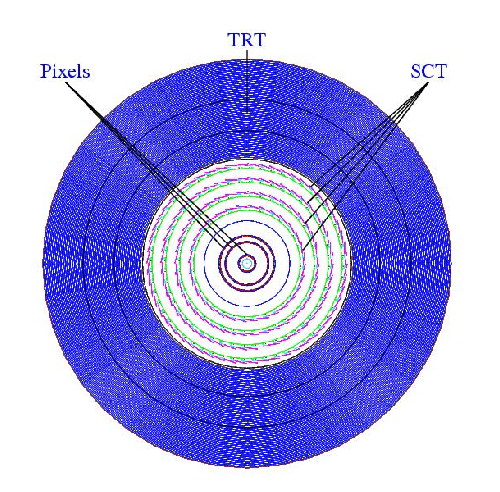
\includegraphics[width=.25\textheight]{capATLAS/innerSection2}\hspace{0.5cm}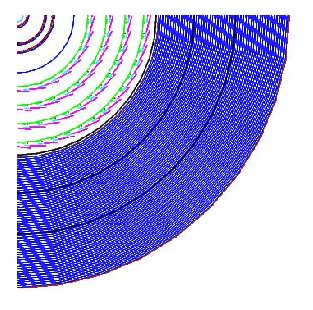
\includegraphics[width=.2\textheight]{capATLAS/innerSection3}\caption{Section of ATLAS inner detector. Each SCT layer has two single sided detectors made of strips parallel to the beam pipe (green) for direct measurement of $\phi$ and rotated (fuchsia) for measurement of the $z$-coordinate.}\label{innersect2}
\end{center}\end{figure} 

Closer to the beam pipe the strips are replaced by silicon pixels of size 50$\times$400 $\mu$m$^{2}$ and with something like 80.4 million readout channels. The pixel detector system has a very high granularity and  provides three precision measurements over the pseudorapidity range $|\eta|<2.5$. Pixel detectors provide very important secondary vertex informations for b-tagging (useful e.g. in bottom and top physics, in the $H \rightarrow b\bar{b}$ decay and in possible decays of supersymmetric particles) thus finding and reconstructing short lived particles such as B-hadrons. For secondary vertex identification the first pixel layer has to be as close to the interaction point as possible. Such layer will probably have to be replaced after some years of running at high luminosity because of radiation damage. Table \ref{tab:sct} shows the intrinsic accuracies of the silicon detectors of the Inner Detector.


\begin{table}[htb]\centering\begin{tabular}{ccccc}
&\multicolumn{2}{c}{Barrel Region} & \multicolumn{2}{c}{End-cap Region}  \\\midrule
&$R-\phi$ plane& $z$-coordinate& $R-\phi$ plane& $R$\\\midrule
Pixel detectors& 10 & 115& 10 & 115 \\\midrule
Strip detectors& 17 & 580 & 17 & 580\\\hline\hline
\end{tabular}\caption{Intrinsic accuracies of Silicon Detectors in $\mu$m.}\label{tab:sct} \end{table}


\subsubsection{Transition Radiation Tracker}
Since semiconductor detectors are quite expensive and add an high amount of material in between the interaction point and the calorimeters, another kind of tracker was choosen to be placed between the silicon tracker and the solenoid. The TRT consists of straw detectors, thin proportional chambers made of straw polyimide drift tubes, 4 mm in diameter. A Xenon based gas mixture is contained in the drift tubes in order to identify electrons since Xenon is sensitive to transition radiation X-rays emitted from  radiator foils placed between the straws. The spatial resolution in the $R-\phi$ plane is 130 $\mu$m per straw, but the high number of position measurements allow to get a final better resolution.

Straws in the TRT are 37 cm long and placed radially in wheels with layers of radiator foils and layers of straws interspaced in the end-cap, while in the barrel region they are 144 cm long and aligned along the beam axis in order to maximise the number of straws crossed by particles coming from the interaction point towards all directions. In the barrel region straws and radiator cannot be put in separate layers because of lack of space. Thus the radiator is formed as sheets of loosely packed polypropylene/polyethylene fibres fitting all available space around the straws. The barrel TRT is also divided into three layers made of chevron shaped modules (Figure \ref{trtmod}). 
\begin{figure}[htb]\begin{center}
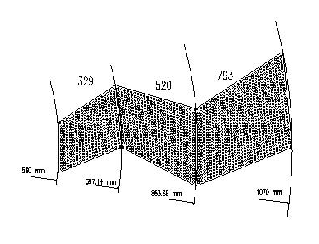
\includegraphics[width=.5\textwidth]{capATLAS/trtmodule}\caption{Modular structure of the barrel TRT. (From \cite{hep})}\label{trtmod}
\end{center}\end{figure}

A total of about 351000 channels compose the electronic readout and each channel provides a drift time measurement with two independent thresholds. This allows the detector to discriminate between particle tracking and transition radiation photons, which pass the lower and the higher threshold respectively. 

So, while the silicon detectors provide in average seven space points on a track with a resolution of few tens of $\mu$m in the $R-\phi$ plane for $|\eta|<2.5$, the TRT gives typically 36 position measurements in the whole pseudorapidity range with a resolution of 130 $\mu$m in the $R-\phi$ plane. Thus the high number of hits and a longer measured track compensate for the worst accuracy of the TRT with respect to SCT, and the combination of the two systems gives highly precise $R-\phi$ and $z$ measurements as well as good pattern recognition.

%The inner detector performance is pivotal for the\dotfill 
%%%%%%%%%%%%%%%%    * Identification of individual particles in dense jets where the calorimeter cannot resolve the individual particles. At the same time the rate of fake tracks should be low.    * Momentum measurement in a large momentum range. Below a transverse momentum of 0.5~GeV the particles loop in the magnetic field and reconstruction is not possible. This lower limit affects the reconstruction of converted photons and J/$\Psi$ decays.    * Charge identification of particles with large transverse momentum for the identification of a possible Z' decay. Increasing the magnetic field will improve the charge identification but at the same time increase the pT limit for loopers.    * Distinguish between electrons and photons which create similar clusters in the EM calorimeter.    * Decay length reconstruction used for CP-violation studies in the B-system and for a Bs0 mixing measurement.    * Tagging of jets originating from high energy b-quarks. The b-jets can be from a H $\rightarrow$ b$\bar{b}$ decay or decays of supersymmetric particles. The tagging is done by secondary vertex identification and through the identification of leptons from semileptonic B-meson decays.    * Electron/jet separation in addition to the separation already provided by the calorimeter.    * Momentum measurement of low energy muons which have large multiple scattering in the hadron calorimeter.    * Identification of the primary vertex in the presence of many vertices from overlying minimum bias events. 
%%%%%%%%%%%%%%%%%Good momentum resolution is provided with a reconstruction of the track along the full track length. This requires both good resolution of the individual detection elements and the possibility to link the individual measurements correctly together to tracks. This pattern recognition problem is treated in more detail in section 6.2.

%In the barrel part of the Inner Detector where |$\eta$| $\lesssim$ 1 all of the detecting elements are ordered in cylindrical structures while the two end-caps have the detecting elements placed in wheels. This assures that the particles pass all detecting elements with large incident angles.



\subsection{Calorimeters}
The superconducting solenoid containing the inner detector is placed inside the electromagnetic calorimeter. Although this choice could affect the energy resolution of the calorimeter because of energy losses\footnote{Particles crossing the material which inner detector and magnet are made of can in fact start showering before reaching the active part of the calorimeter.}, the advantage is a compact design and a lower transverse spread of showers thanks to the absence of magnetic field.

The distinction between electromagnetic and hadronic calorimeters is due to the different phenomenology of the physics involved. The development of electromagnetic showers from an incident electron or photon is well understood and for particles with equal incident energy the variations in shape and measured energy of the showers are quite small. The size of the shower is linearly dependent on the radiation length $X_{0}$ of the material entered, while the size of hadronic showers depends linearly on the nuclear interaction length\footnote{The nuclear interaction length is the average distance traveled by hadrons before inducing a nuclear reaction.} $\lambda_{int}$ of the material. 

%The hadronic and electromagnetic showers profiles look on average very similar, except for the fact that $X_{0}$ is much lower than $\lambda_{int}$. Besides the behaviour of hadrons in the calorimeter material is quite different since the nuclear processes involved show large variations in the amount of energy transferred to secondary particles of the shower (pions at the 90\%). Neutral pions decay in two photons, thus starting electromagnetic showers that, in the end, will carry about the 30-50\% of the total of the hadronic shower energy. The non-electromagnetic energy is mainly deposited through nucleons (ionising particles from protons, neutrons and invisible energy\footnote{The so called \textit{invisible energy} accounts from the binding energy provided to the nuclear environment in order to release the nucleons, thus is not revealed in the calorimeter.}), resulting in the non compensation phenomenon: the calorimeter signals for pions are generally lower than signals from electrons of the same energy. Since the electromagnetic fraction of the hadronic shower is energy dependent (and increases with energy), also the electron/pion response ratio $e/\pi$ ($>1$) will be. The ratio between signals from purely electromagnetic and purely hadronic part of the shower is called $e/h$ and characterizes the degree of non compensation. The relation between these ratios is expressed by the formula \begin{equation}\label{eq:ehratio}\dfrac{e}{\pi} = \dfrac{e/h}{1 - f_{em}(1- e/h)},\end{equation} where $f_{em}$ is the electromagnetic fraction of the shower, thus energy dependent; compensating calorimeters try to make the $e/h$ ratio as close as possible to one.

In order to separate electromagnetic showers from hadronic showers it is useful to consider the huge difference between $X_{0}$ and $\lambda_{int}$, that for materials whith high $Z$ number can be as large as a factor of 30. High density materials mean a compact calorimeter, but low $Z$ materials, with similar interaction and radiation length, can minimise the fluctuations in the response for the hadronic calorimeter. 

The need of rejecting QCD jets faking electrons and photons at the level of $10^{6}$ and $10^{3}$ respectively %in order to have clean signals of electrons with $p_{T}>20$~GeV 
is reflected by the fine granularity in both the electromagnetic and hadronic part of the calorimeter. This allows to identify isolated energy depositions from electromagnetic showers excluding signals that expand behind the electromagnetic calorimeter. 
%Identification of electrons and photons are the most important issues for the calorimeters. The rate of QCD-jets is high and to be able to get a clean sample of electrons with transverse momentum above 20~GeV a rejection of QCD-jets at the level of 106 is required. Such a rejection can be achieved with a calorimeter of fine granularity in both the EM and hadronic part to identify isolated energy depositions from electrons/photons and to veto on hadronic energy behind the cluster in the EM calorimeter.

Good hermeticity instead is required to identify missing transverse energy as signal from undetectable particles like neutrinos and expected supersymmetric particles. Thus the pseudorapidity range has to reach $|\eta|$ = 5 being aware of minimising possible discontinuities (e.g. cables and cooling system) in the detector. For the hadronic calorimeter this is even more important because the leakage of hadrons from it would provide background into the muon system besides a worst missing transverse energy.

The compromise between the total size of the ATLAS detector, the choice of materials for discrimination between electromagnetic and hadronic showers still having low fluctuations in the energy response, the need of having muons reaching the muon system and a good resolution in missing transverse energy, is finally found in making the electromagnetic calorimeter more than 22$X_{0}$ in the barrel region and more than 24$X_{0}$ in the end-caps thick and the hadronic calorimeter 11$\lambda_{int}$ thick (including the outer support material) at $\eta=0$. The calorimeter has a barrel region divided into a small electromagnetic sampling calorimeter (sharing the cryostat with the superconducting solenoid of the inner detector) closer to the beam pipe and with high resolution, and a hadronic tile calorimeter around it with a coarser resolution (Figure \ref{caloBarrel}). In the end-cap region there are electromagnetic and hadronic sampling calorimeters, embedded in cryostats, and in the pseudorapidity region $3.1 < |\eta| < 4.9$ there is another sampling calorimeter, called \textit{very forward}. These end-cap and very forward calorimeters are embedded in the tile extended barrel calorimeter and the whole structure is contained in a cylindrical support.

In the pseudorapidity range $|\eta|<2.5$ measurements from calorimeters are matched with measurements from the inner detector, thus fine granularity allows electrons and photons precise measurements. In the rest of the range instead coarser granularity is still suitable for measurements of the missing transverse energy and jet reconstruction.

\begin{figure}[htb]\begin{center}
\includegraphics[width=.95\textwidth]{capATLAS/caloBarrel}\caption{ATLAS calorimeters. }\label{caloBarrel}
\end{center}\end{figure}



%In line with the coverage for the detection of electrons and muons in the calorimeter and muon system the coverage of the Inner Detector extends up to |$\eta$| = 2.5 .
% In the forward direction it reaches down to $\eta$ = 3.2 . 

\subsubsection{Electromagnetic calorimeter}
The electromagnetic calorimeter consists of a liquid argon (LAr) sampling calorimeter with a design optimized for the requirements in energy and spatial resolution for the Higgs decays involving electrons or photons as signatures. The energy range for electrons and photons is from 2~GeV (i.e. from bottom quark semi-leptonic decay) up to a few TeV (i.e. from vector bosons decays). 
%The $H \rightarrow\gamma\gamma$ decay of a standard model Higgs has a large background and a mass resolution around 1\% is required (see chapter 7). The dynamic range for the calorimeter ranges in transverse energy from around 1~GeV for electrons from B-meson decays to a few TeV for the decay of a heavy vector boson.
The electromagnetic calorimeter has a barrel part ($|\eta| < 1.475$) more than 22$X_{0}$ thick and two end-cap regions ($1.375 < |\eta| < 3.2$) more than 24$X_{0}$ thick. Layers of active and passive material (LAr and lead respectively) are disposed as shown in Figure \ref{caloLAr2}. 
%The lead gives the shower development with its short radiation length and the secondary electrons create ionisation in the narrow gaps of liquid argon. An inductive signal from the ionisation electrons drifting in the electric field across the gas-gap is registered by copper electrodes. 
Such accordion shape of the lead plates allows a fast response (low capacitance of the detecting elements) and homogeneousity in the $\phi$ coordinate. The segmentation is both longitudinal and transverse and the barrel calorimeter is divided in depth in four samplers: one presampler and three layers (front, middle and back). 

\begin{figure}[htb]\begin{center}
\includegraphics[width=.55\textwidth]{capATLAS/caloLAr2}\caption{LAr sampling calorimeter (barrel calorimeter): lateral and longitudinal segmentation. (From \cite{Aad:JINST})}\label{caloLAr2}
\end{center}\end{figure}

The presampler, closest to the interaction point, consists of only LAr, with no layer of assorbing material, with the aim of correcting for the energy loss of particles crossing the inner detector, the solenoid and the cryostat wall. It is divided into 64 identical azimuthal sectors which cover a region $\Delta\eta\times\Delta\phi$ = 1.52$\times$0.2.

The first sampling (front layer) is 4.3$X_{0}$ thick with thin readout strips ($\Delta\eta\times\Delta\phi$ = 0.0031$\times$0.098) providing an excellent resolution in $\eta$. Measurements of $\eta$ helps for photon/$\pi^{0}$ separation while the $\phi$ coordinate does not provide useful informations since converted photons, opening up in the magnetic field, produce clusters with widths similar to $\pi^{0}$ ones.

The second sampling (middle layer), 16 radiation lengths thick, collects the majority of deposited energy and is able to fully contain clusters with energy up to 50~GeV. It is divided in towers with dimension $\Delta\eta\times\Delta\phi$ = 0.025$\times$0.0245, providing position measurement of the cluster. The energy of the shower is deposited for the 95\% in a matrix of 3$\times$7 towers $\Delta\eta\times\Delta\phi$.

Finally, the third sampling (back layer) is going to receive only the highest energy electrons belonging to wide clusters. Thus the towers dimension is now doubled in $\eta$ ($\Delta\eta\times\Delta\phi$ = 0.05$\times$0.0245) without losing in resolution.

End-cap calorimeters cover the range $ 1.375 < |\eta| < 3.2$ with a LAr presampler at $1.5<|\eta|<1.8$ devoted to improve the bad energy resolution due to the discontinuity between barrel and end-cap calorimeters. Furthermore end-cap calorimeters are divided into two coaxial wheels, one internal for $ 2.5 < |\eta| < 3.2$ and one external for $1.375 < |\eta| < 2.5$ separated by 3 mm of material. Also end-cap calorimeter are segmented in depth, in three layers for the precision region $1.5 < |\eta| < 2.5$ and in two layers for the inner wheel and for the outer wheel in the region $1.375 < |\eta| < 1.5$.

The resolution of a sampling calorimeter, with energies measured in~GeV, is given by the equation
\begin{equation}\label{eq:resolution}
\frac{\Delta E}{E} = \frac{a}{\sqrt{E}}\oplus\frac{b}{E}\oplus c,
\end{equation} where the terms of the sum are, respectively, statistical (considering shower development), instrumental (consisting of readout electronic rumor effects) and systematic (depending on calibration, shower containment, inactive material etc). Approximately, the numerical values for factors $a, b$ and $c$ give
\begin{equation}\label{eq:resolution2}
\frac{\Delta E}{E} = \frac{10\%}{\sqrt{E}}\oplus\frac{300\mbox{ MeV}}{E}\oplus 0.5\%.
\end{equation}
%The sampling term a is defined by the number of lead/argon interfaces and is 8-11% depending on rapidity. Noise influences the resolution at the lowest energies through the term b which is of the order 400 MeV when running at high luminosity. The constant term affects the resolution for high energy clusters and is limited by the calibration of the global energy scale and local variations in this. It is hard to predict but is believed to stay below 0.7%[*].

\subsubsection{Hadronic calorimeter}
The barrel hadronic calorimeter is a tile calorimeter that covers (thanks to the two extended barrels in $0.8<|\eta|< 1.7$) the pseudorapidity region $|\eta|< 1.7$. The design of the tile calorimeter is shown in Figure \ref{caloTile}: steel absorbers are arranged in a matrix with scintillator tiles placed on parallel layers and slightly rotated in order to make showers cross them from the side. Light signals from scintillators is sent to photomultipliers outside of the calorimeter through wavelength shifting fibres. The tile barrel and extendex barrel calorimeters are both segmented in depth in three layers.

\begin{figure}[hbt]\begin{center}
\includegraphics[width=.4\textwidth]{capATLAS/caloTile}\caption{Tile calorimeter component. (From \cite{Aad:JINST})}\label{caloTile}
\end{center}\end{figure}
%To improve the hermicity of the hadronic calorimeter two plugs in each side are inserted in the region where the cables and cooling from the EM calorimeter and the Inner Detector pass through. One of them, the crack scintillator, is a pure scintillator with no steel absorber. This design is forced by the limited space in the region. It plays an important role for the EM calorimeter as well since it is placed just in the difficult transition region between the barrel and end-cap EM calorimeter. 

At $1.5<|\eta|<3.2$ there are the hadronic end-cap calorimeters (HEC), LAr sampling calorimeters like the electromagnetic calorimeters with which they share the cryostat. End-cap calorimeters are formed by two wheels each, segmented in two layers in depth, with parallel copper plates placed perpendicular to the beam, acting as assorbers.

In the very forward region, the forward LAr calorimeter FCal is both electromagnetic (module with copper absorbers) and hadronic (two modules with tungsten absorbers) and minimise the transverse development of showers. It is a matrix of absorber material with cylindrical holes where the active material is placed. The quantity of liquid argon is low (the gap between absorbers is just 250 $\mu$m) in order to have fast readout and limited sensitivity to pile-up effects.


%The reconstruction of jets is important for studies of quark compositeness. This sets stringent limits on the linearity of the hadronic calorimeter response at high energies. Also for the reconstruction of W bosons in hadronic decays the jet energy resolution is important as discussed in detail in chapter 8.
The resolution of the tile calorimeter for $|\eta|<3$ is
\begin{equation}\label{eq:resolutionTile}
\frac{\Delta E}{E} = \frac{50\%}{\sqrt{E}}\oplus 3\%,
\end{equation} with a segmentation of $\Delta\eta\times\Delta\phi = 0.1\times0.1$, while in the region $3<|\eta|<4.9$ where coarser segmentation and lower precision is needed the resolution is
\begin{equation}\label{eq:resolutionTile2}
\frac{\Delta E}{E} = \frac{100\%}{\sqrt{E}}\oplus 10\%.
\end{equation} The constant term is mainly depending on the non compensation between the response to the hadronic and electromagnetic part of the shower.


\subsection{Muon Spectrometer}
Because of the high multiplicity of tracks, a stand alone system for muon identification and $p_{T}$ measurements is needed. The design of the calorimeters is such that muons are the only particles escaping the high amount of material and thus reaching the muon system (Figure \ref{muonsDrift}). This system, surrounding the whole of the internal detectors and the air-core toroidal magnets, is a precision muon spectrometer and a trigger for high energy muons events ($H\rightarrow ZZ^{(*)}\rightarrow4\mu$).

\begin{figure}[hbt]\begin{center}
\includegraphics[width=.8\textwidth]{capATLAS/muonsDrift}\caption{Muon system.}\label{muonsDrift}
\end{center}\end{figure}

The superconducting air-core toroid magnet has an open structure with eight superconducting toroidal coils with separate cryostats in the barrel part while in the end-cap regions is made of eight coils sharing the cryostat. The field strength varies strongly with $\phi$, making field integral $\int Bdl$ in the barrel region ($|\eta|<1.4$) 1.5-5.5 Tesla$\cdot$m and in the end-caps ($1.6<|\eta|<2.7$) 1-7.5 Tesla$\cdot$m. In the so-called transition region $1.4<|\eta|<1.6$, magnetic deflection results from a combination of the two fields. Such configuration of the magnets gives a field perpendicular to muon tracks. The complex of the magnet system is shown in Figure~\ref{magnets}
\begin{figure}[hbt]\begin{center}
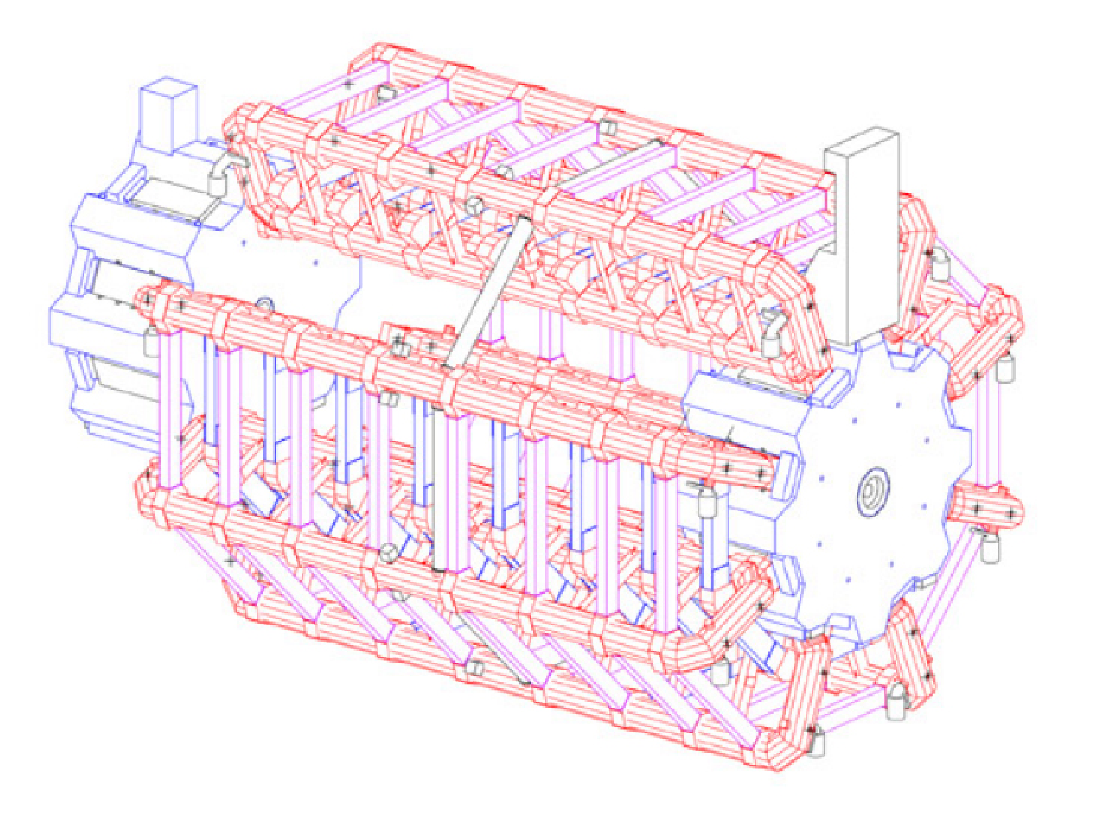
\includegraphics[width=.8\textwidth]{capATLAS/magnets}\caption{Magnet system.}\label{magnets}
\end{center}\end{figure}

%Since the magnetic field has several inhomogeneity it is important to measure the R$\phi$ coordinate with a precision of centimeter. 
The muon system has three sets of detectors composed of MDT (Monitored Drift-Tube) chambers, Cathode Strips Chambers (CSC), Resistive Plate Chambers (RPC) and Thin Gap Chambers (TGC) placed with different layouts in the barrel and end-cap regions. The barrel region is instrumented with chambers arranged in three cylindrical layers around beam axis with one layer inside the magnet, while in the end-caps these three layers are placed perpendicular to the beam axis (Figure \ref{muonSect}).

\begin{figure}[hbt]\begin{center}
\includegraphics[width=.4\textwidth]{capATLAS/muonSect2}\includegraphics[width=.5\textwidth]{capATLAS/muonSect}\caption{Left: cross section of the barrel muon system. Right: lateral section of the muon system. Barrel MDTs are shown in green, end-caps MDTs in light blue, CSC in yellow, TGCs in magenta, RPCs in white.  (From \cite{Aad:JINST})}\label{muonSect}
\end{center}\end{figure}


\subsubsection{Monitored Drift Tubes (MDT)}
MDTs are present on all layers both in the barrel and end-cap regions and are precision chambers to measure the coordinate in the bending plane of the magnet. They are proportional chambers constituted by drift tubes with a diameter of 30 mm and lenght varying from 0.9 m to 6.2 m. In the pressurised drift tubes (29.97 mm in diameter) the gas mixture, kept at 3 bars, is 93\% Ar and 7\% CO$_{2}$ and a central tungsten-rhenium wire (50 $\mu$m in diameter) collects electrons coming from ionisation. Drift tubes are placed transverse to the beam axis and each set is made of 2 superlayers each with 3 or 4 layers of tubes (Figure \ref{mdt}). With such a high number of tubes MDTs allow for a very good track reconstruction and high reduction of the fake tracks from random associations of background hits. The resolution of 80 $\mu$m gives a momentum resolution $\Delta p_{T}/p_{T} < 10^{-4}$~GeV$^{-1} \cdot p_{T}$ for tracks with $p_{T} > $300~GeV.% Tracks with lower transverse momentum have a resolution limited by multiple scattering and stopping power of the hadron calorimeter.
\begin{figure}[hbt]\begin{center}
\includegraphics[width=.7\textwidth]{capATLAS/mdt}\caption{Single MDT set from the barrel region. End-caps MDTs are trapezoidal instead of rectangular but keep the same structure shown. (From \cite{Aad:JINST})}\label{mdt}
\end{center}\end{figure}


\subsubsection{Cathode Strip Chambers (CSC)}
CSCs, the other precision chambers, take the place of MDTs in the forward region $|\eta|>2$ since there MDTs cannot withstand the high particle flux. The CSCs are arranged in a system of two disks with eight chambers each. These chambers contain four CSC planes each one giving independent measurements of $\eta$ and $\phi$ along the tracks. A CSC is a multiwire proportional chamber with wires oriented in the radial direction and spaced of 2.5 mm in a gas mixture of Ar (80\%) and CO$_{2}$ (20\%). Cathode strips are both segmented, one is arranged perpendicular to the anode wires giving the precision coordinate, while the other is parallel to the wires, thus providing the transverse coordinate. The position measurement comes from the interpolation between the charges induced on neighbouring cathode strips, with a provided resolution of 50 to 70 $\mu$m.

\subsubsection{Resistive Plate Chambers (RPC)}
Drift tubes cannot be used for trigger purpose since their large diameter results in a maximum drift-time of 500 ns, too long with respect to the 25 ns spacing of the bunch crossings. Thus special layers of trigger chambers are implemented and combined to MDTs and CSCs. In the barrel region the MDT's second layer is covered on both sides by RPCs, while MDT's third layer is covered by a RPC alternatively on the inner and outer side. In the end–caps, RPCs cover the inner side of MDT's first and third layers.

A RPC is a detector with a gas-gap between two resistive bakelite plates, kept parallel to each other at a distance of 2 mm in a gas mixture made of C$_{2}$H$_{2}$F$_{4}$ (94.7\%), Iso-C$_{4}$H$_{10}$ (5\%) and SF$_{6}$ (0.3\%). The uniform electric field between the plates forms avalanches along the ionising tracks towards the anode and the signal is read out by two orthogonal sets of pick-up strips providing a position resolution of 1 cm in each plane and a 1 ns time resolution. This allows to discriminate between individual bunch crossings. RPCs with this lower spatial resolution provide a sufficient momentum resolution and the $\phi$ coordinate for the tracks in the final analysis since MDTs only give the $\eta$ coordinate.

\subsubsection{Thin Gap Chambers (TGC)}
Since RPCs can withstand a maximal flux of 1 Hz$\cdot$cm$^{-2}$, they are replaced with TGCs in the $|\eta|>1.05$ region. TGCs are similar to CSCs, have 1.8 mm wire-to-wire separation and 1.4 mm wire-to-cathode separation and provide a time resolution of 5 ns. The highly quenching gas mixture (CO$_{2}$ 55\% and n-C$_{5}$H$_{12}$ 45\%) prevents the occurence of streamers. With a spatial resolution of about 1 mm, TGCs are used for trigger signal as well as for $\eta$ and $\phi$ coordinates informations.

%In the most compact and cost efficient way the design of the muon system has to fulfil a set of conditions:
%    * A good transverse momentum resolution in the low pT region. The limit is defined by the ability to detect the H $\rightarrow$ ZZ * decay in the muon channel with a high suppression of the background. A resolution of around 1% is required for this.    * At the highest pT the muon system should have sufficient resolution to give good charge identification for an identification of a Z' $\rightarrow$ $\mu$$\mu$ decay.    * A rapidity coverage |$\eta$| < 3 . A smaller rapidity coverage will strongly reduce the number of events with a high mass object decaying to muons with all muons inside the covered region.    * A hermetic system to prevent particles to escape through holes.    * Measurement of spatial coordinates in 2 dimensions to provide good mass resolution.    * A low rate of both punch through hadrons and fake tracks.    * A trigger system for almost all physics channels. The requirement on rapidity coverage is similar to the requirement for the main muon system. For B-physics a maximal coverage for muons with transverse momentum down to 5~GeV is desirable. 

\subsection{Trigger and Data Aquisition}
Because of the huge amount of data coming from each bunch crossing at the frequency of 40 MHz, a severe on-line event selection system is needed. Since it is only possible to write events to tape at a rate about 200 Hz, the ATLAS trigger system has to reduce the data flow by a factor of 2$\cdot10^{5}$; this is done with a three level trigger system (Figure \ref{trigger1}).

\begin{figure}[hbt]\begin{center}\begin{minipage}{.45\textwidth}
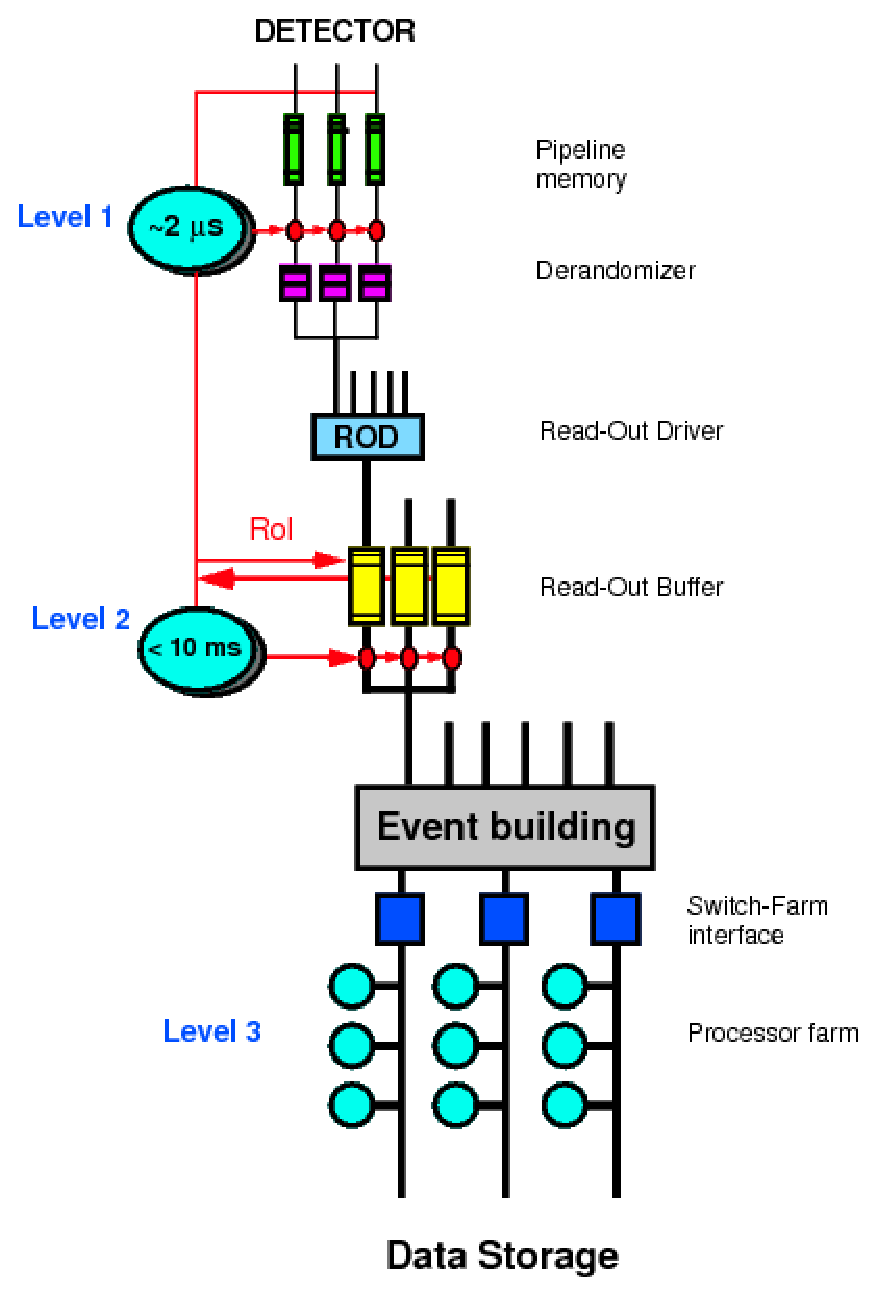
\includegraphics[width=.99\textwidth]{capATLAS/trigger1}
\end{minipage}\begin{minipage}{.55\textwidth}
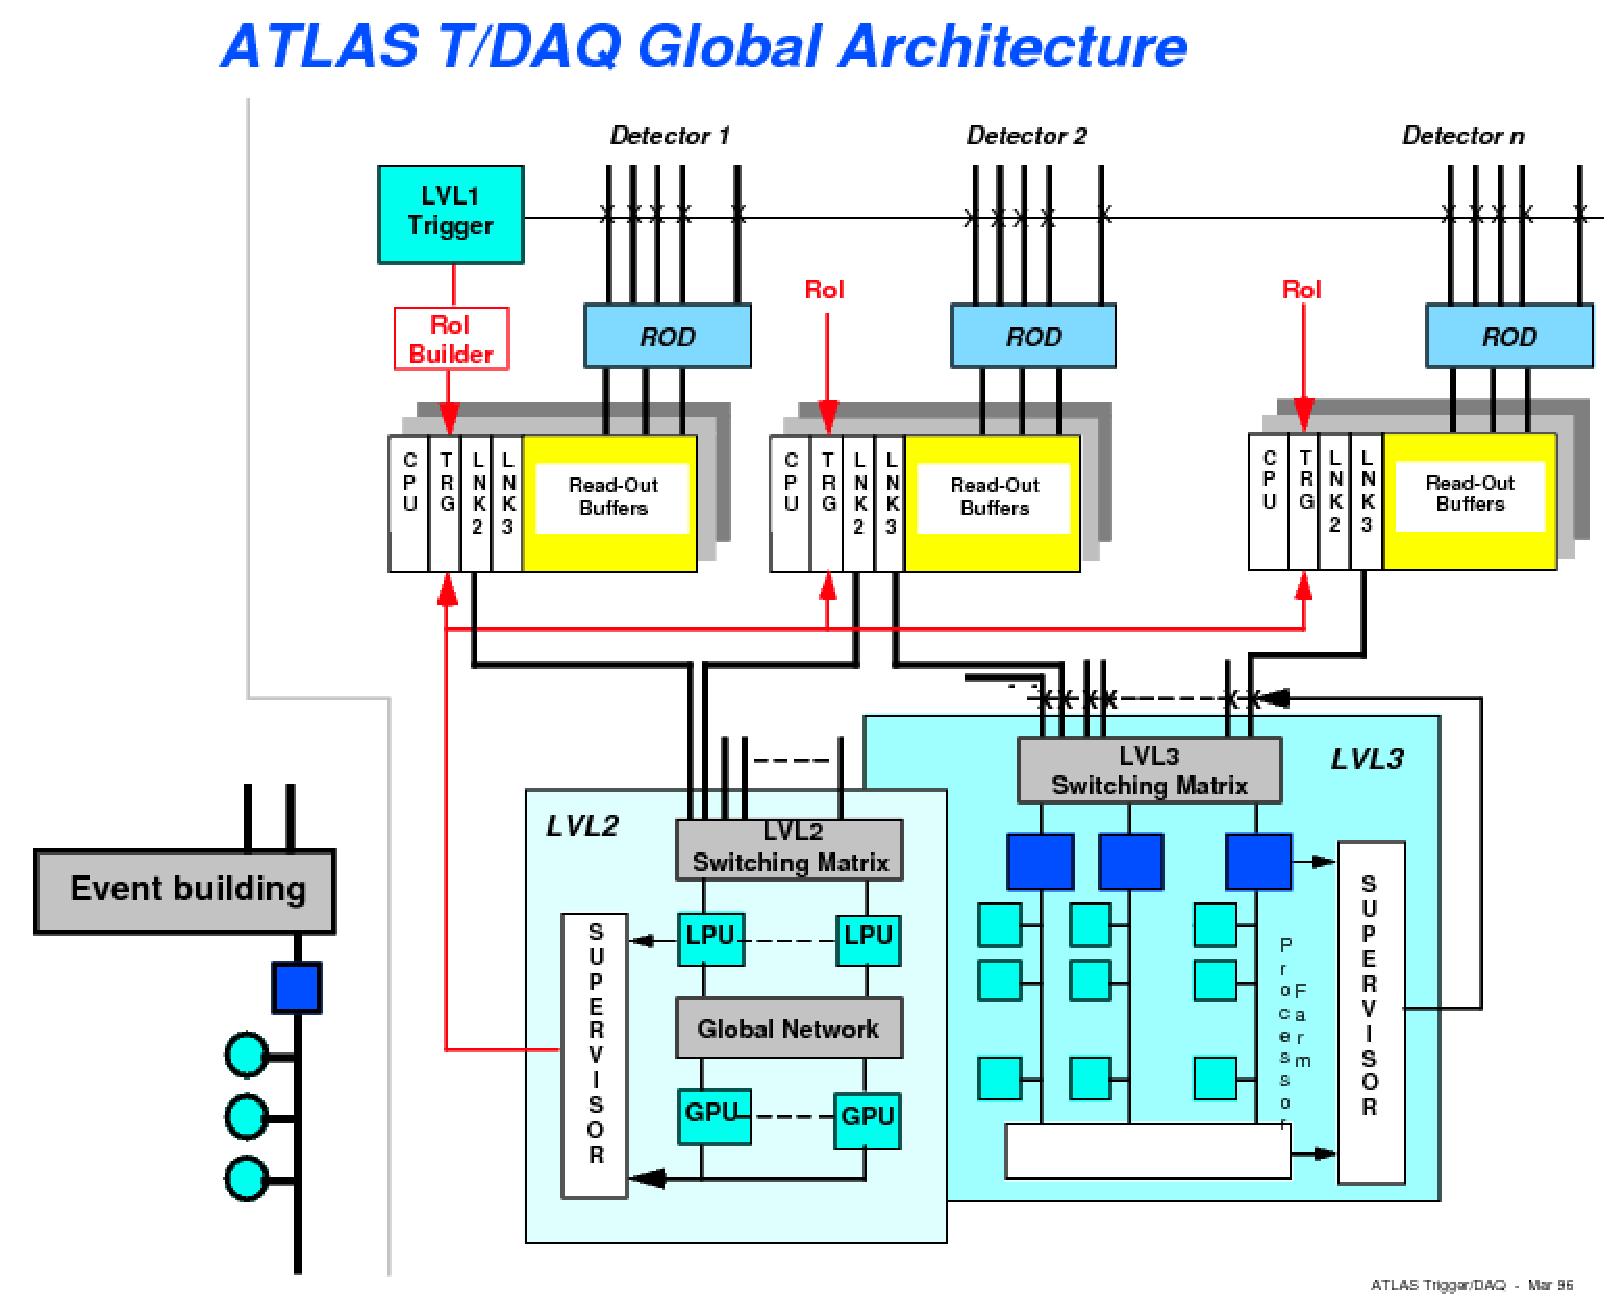
\includegraphics[width=.99\textwidth]{capATLAS/trigger2}
\end{minipage}
\caption{Trigger scheme. }\label{trigger1}
\end{center}\end{figure}

Each level introduces appropriate selection rules to refine informations from the previous trigger level. Level-1 trigger (LVL1) collects data from calorimeters and muon system only that are read out with a coarse resolution  $(\Delta\eta\times\Delta\phi = 0.1 \times 0.1)$ and a fast processing time (less than 2.5 $\mu$s to reach its decision\footnote{This time includes propagation delays due to cables, since signal has to travel from the detector to the underground counting room where the trigger logic is housed.}). All informations from detectors have to be stored in pipeline memories until the LVL1 decision is available. LVL1 trigger selects the so-called Regions of Interest (RoI, Figure \ref{trigger3}) characterized by isolated electromagnetic clusters with $E_{T} > 30$~GeV, large missing transverse energy, high energy jets, muons with $p_{T} > 20$~GeV, but more complicated and different triggers also exist\footnote{With low luminosity, B-physics programs will require specific triggers, like a LVL1 trigger for isolated muons with $p_{T} > 6$~GeV.}.% and at level-2 a J/$\Psi$ trigger in the TRT. This J/$\Psi$ trigger will not run inside a small region of interest but cover the entire TRT. The electron identification power of the TRT is important for this trigger to reject random combinations of hadrons from faking J/$\Psi$'s.} .
%The trigger algorithms are changeable and will to some extent be adjusted after data taking has started reflecting the present uncertainties in the minimum bias structure. An isolated cluster means that a region  ($\Delta$$\eta$ x $\Delta$$\varphi$) around the central cluster contains low transverse energy.
%More complicated triggers requiring two or more clusters/tracks also exists, an example of this is the trigger used for the H $\rightarrow$ $\gamma$$\gamma$ decay which requires two isolated electromagnetic clusters with ET > 20~GeV. All data is stored on the detector in pipelines of the readout electronics waiting for a trigger level-1 decision. After a fixed delay the data is either lost or read out by a trigger level-1 accept signal.

Then, events selected by the LVL1 trigger are sent to the level-2 trigger (LVL2), waiting in read out buffers (ROB) for the LVL2 decision which takes about 40 ms, processing many events in parallel. LVL2 trigger uses full precision informations from all detectors (including the inner detector) in the RoIs indicated by LVL1, reducing the 100 kHz rate from LVL1 of a factor $10^{2}$. 
%The analysis takes place in a region, a so-called Region of Interest, around the direction in ($\eta$,$\varphi$) selected by the level-1 trigger. The main task of the level-2 trigger is to refine the analysis of the level-1 trigger inside this region of interest. Taking as an example again the H $\rightarrow$ $\gamma$$\gamma$ decay, the trigger level-2 analysis calculates the cluster energy with the full resolution to refine the isolation cut. Jet events with energy deposition in the hadronic calorimeter behind the electromagnetic cluster are also rejected. In total this reduces the rate in the two photon trigger by a factor 25 with only a small loss of efficiency.
%The Inner Detector is also involved in the level-2 trigger. For the isolated electron trigger the Inner Detector searches for tracks pointing towards the cluster. For electrons the pT of the most energetic track should loosely match the ET of the cluster.
1 kHz is the highest acceptable rate for the event builder, which from LVL2 data applies more complicated physics analysis. The event builder collects the limited informations about small parts of subdetectors for a single event contained in each readout buffer and send them to the event filter (EF) in the process of data aquisition (DAQ). EF achieve the 200 Hz limit for event rate, the highest acceptable rate for data storage, performing event building on events selected by LVL2 trigger.
%The level-3 trigger analyses data in the full detector and will do more complicated physics analysis. Many physics channels will be covered by a trigger for Z $\rightarrow$ l +l - decays with a tight invariant mass cut around the Z mass. The H $\rightarrow$ $\gamma$$\gamma$ decay is problematic at this trigger level since it will be required to store all events with a two photon invariant mass above 60~GeV or so. A strong rejection of $\pi^{0}_{}$ 's faking photons is necessary for this. The level-3 trigger will reduce the data rate down to 100 Hz which is the highest acceptable rate for permanent storage of data.
%The trigger system is sensitive to the theoretical uncertainties of the background levels to the physics channels. For this reason a factor two safety limit is build into the level-1 trigger where all thresholds are fully adjustable. For the level-2 trigger all analysis is programmable allowing for changes and upgrades of the software after the start of the LHC. For the level-3 trigger which will be based on standard workstations/PC's even the hardware can be upgraded to take advantage of the improved performance on the market. 

%Event Filter and Data Aquisision
%For LVL2-selected events, event building is performed. Each readout buffer contains fragments of many events for a small part of one subdetector. The event builder collects all the fragments from one event into a single memory - the memory of an Event Filter processor. The event building is performed using a data switch.
%Event Filter processing is performed using farms of processors acting on the full-event data. The complicated selection criteria of the off-line analysis will be used in a real-time environment. The processing time per event could be about 1 second on a 1000 MIPS (Million Instructions Per Second) processor (today's processors are typically 100-200 MIPS)
%The figure above shows, on the left, a fuctional view of the trigger and DAQ systems, on the right is an implementation view emphasising the trigger levels and their interaction with the DAQ system.

\begin{figure}[hbt]\begin{center}\begin{minipage}{.45\textwidth}
\includegraphics[width=.95\textwidth]{capATLAS/Roi}
\end{minipage}\hspace{.05\textwidth}\begin{minipage}{.45\textwidth}
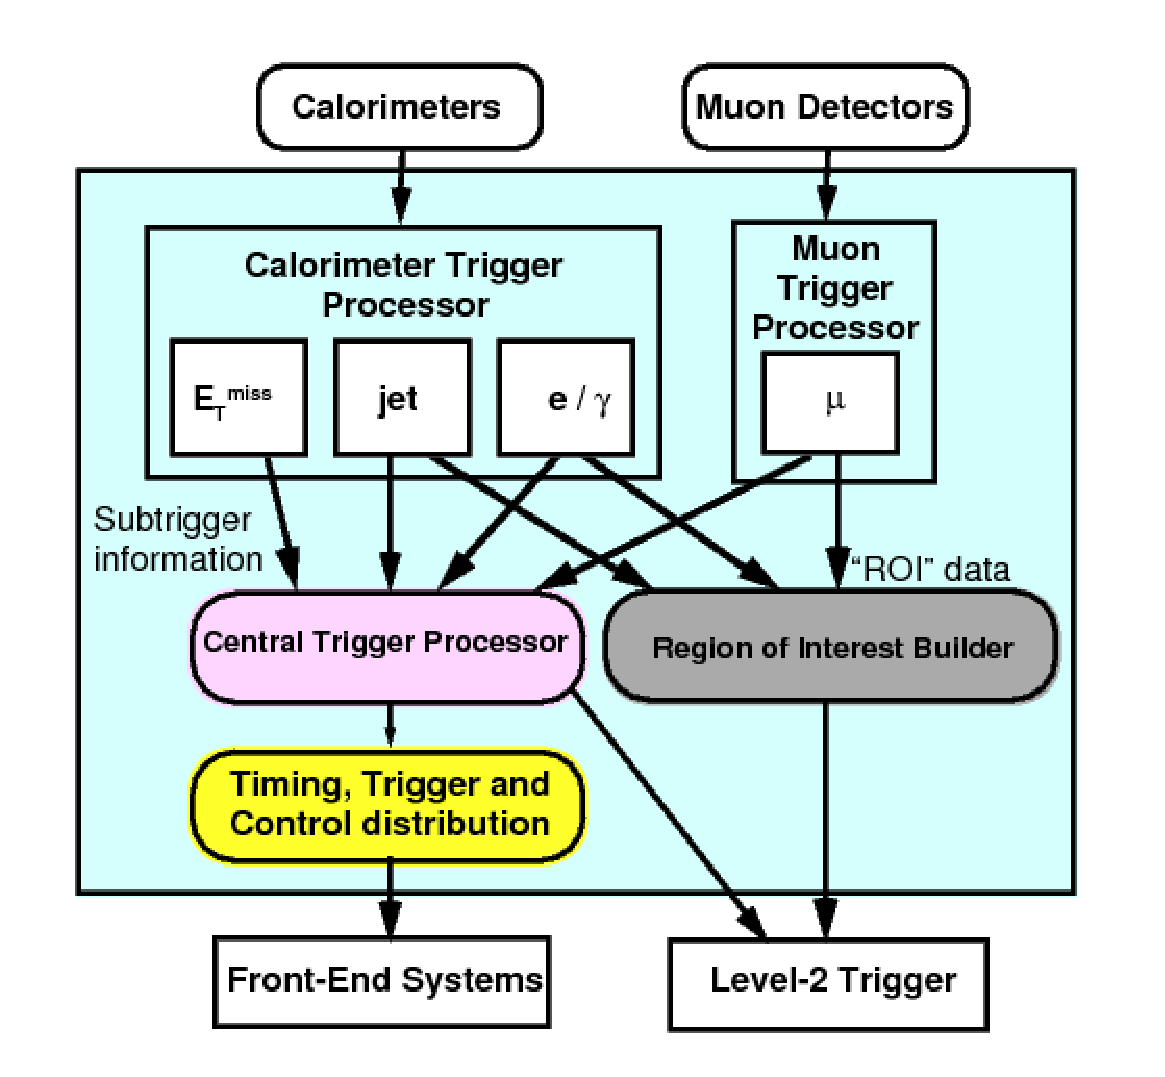
\includegraphics[width=.9\textwidth]{capATLAS/trigger3}
\end{minipage}
\caption{Regions of Interest (left) and trigger scheme (right). }\label{trigger3}
\end{center}\end{figure}


%DAQ prototype "-1"
%A project is in progress to study the full fuctionality of the DAQ and Event Filter systems.
%The goal of this project is to produce a prototype system representing a "full slice" of a DAQ system, and suitable for evaluating candidate technologies and architectures for the final ATLAS DAQ system.
%Work started on defining the requirements in Spring 1996 and it is expected that the prototype will be running in 1998. Each phase of the project is reviewed by the ATLAS Trigger/DAQ community.

%---------------------------------------------------
%---------------------------------------------------
%-----   COPY UP TO HERE TO DEFINITIVE FILE   ------
%---------------------------------------------------
%---------------------------------------------------
